\documentclass[12pt]{article}
\setlength{\oddsidemargin}{0in}
\setlength{\evensidemargin}{0in}
\setlength{\textwidth}{6.5in}
\setlength{\parindent}{0in}
\setlength{\parskip}{\baselineskip}
\usepackage{amsmath,amsfonts,amssymb}
\usepackage{graphicx}
\usepackage{enumitem}
\usepackage[]{algorithmicx}
\usepackage{amsthm}
\usepackage{fancyhdr}
\pagestyle{fancy}
\setlength{\headsep}{36pt}
\usepackage{tkz-berge}
\usetikzlibrary{positioning, automata}

\usepackage{hyperref}

\theoremstyle{remark}
\newtheorem*{solution}{Solution}

\newcommand{\makenonemptybox}[2]{%
%\par\nobreak\vspace{\ht\strutbox}\noindent
\item[]
\fbox{% added -2\fboxrule to specified width to avoid overfull hboxes
% and removed the -2\fboxsep from height specification (image not updated)
% because in MWE 2cm is should be height of contents excluding sep and frame
\parbox[c][#1][t]{\dimexpr\linewidth-2\fboxsep-2\fboxrule}{
  \hrule width \hsize height 0pt
  #2
 }%
}%
\par\vspace{\ht\strutbox}
}
\makeatother

\begin{document}
\definecolor {processblue}{cmyk}{0.96,0,0,0}

\lhead{{\bf CSCI 3104, Algorithms \\ Problem Set 5a (11 points)} }
\rhead{Name: \fbox{Michael Rogers} \\ ID: \fbox{105667404} \\ {\bf Profs.\ Hoenigman \& Agrawal\\ Fall 2019, CU-Boulder}}
\renewcommand{\headrulewidth}{0.5pt}

\phantom{Test}

\begin{small}
\textbf{Instructions for submitting your solution}:
\vspace{-5mm} 

\begin{itemize}
	\item The solutions \textbf{should be typed} and we cannot accept hand-written solutions. \href{http://ece.uprm.edu/~caceros/latex/introduction.pdf}{Here's a short intro to Latex.}
	\item You should submit your work through \href{https://www.gradescope.com/courses/59294}{\textbf{Gradescope}} only.
	\item If you don't have an account on it, sign up for one using your CU email. You should have gotten an email to sign up. If your name based CU email doesn't work, try the identikey@colorado.edu version. 
	\item Gradescope will only accept \textbf{.pdf} files (except for code files that should be submitted separately on Gradescope if a problem set has them) and \textbf{try to fit your work in the box provided}. 
	\item You cannot submit a pdf which has less pages than what we provided you as Gradescope won't allow it. 
	\item Verbal reasoning is typically insufficient for full credit. Instead, write a logical argument, in the style of a mathematical proof.
	\item For every problem in this class, you must justify your answer:\ show how you arrived at it and why it is correct. If there are assumptions you need to make along the way, state those clearly.
	
	\item You may work with other students. However, \textbf{all solutions must be written independently and in your own words.} Referencing solutions of any sort is strictly prohibited. You must explicitly cite any sources, as well as any collaborators. 
\end{itemize}



\vspace{-4mm} 
\end{small}

\hrulefill

\newpage
\begin{enumerate}
%\item (2 pt) Use the following graph $G$ to describe the difference between an MST and the single-source shortest path in a graph. Your answer should clearly describe the different trees that Kruskals and Dijkstras algorithms produce on $G$. 
\item (7 pts) Consider the following weighted graph. 
\begin{figure}[h!]
\begin{center}
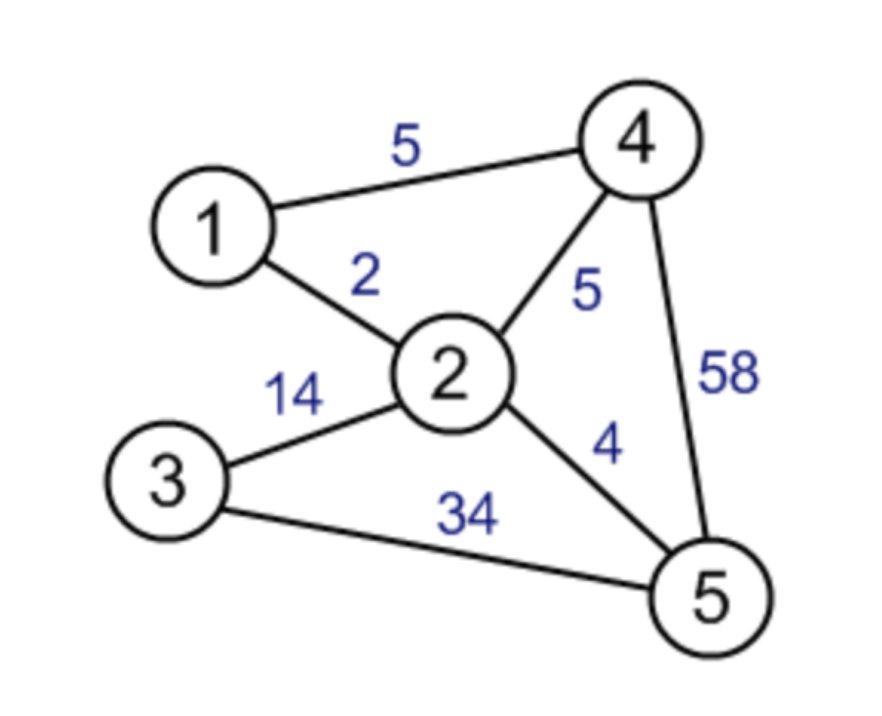
\includegraphics[scale=0.3]{PS5aQ1.png} 
\end{center}
\end{figure}

\begin{enumerate}[label=(\alph*)]
\item (2 pts) Run Dijkstra's algorithm on this graph to obtain a tree of shortest paths. Use vertex $1$ as the source vertex.
\begin{solution}
Table of Solved Verticies
\begin{center}
\begin{tabular}{ |c|c|} 
 \hline
 Verticy & Shortest Path from 1 \\ 
\hline
 1 & 0 \\ 
 2 & 2 \\ 
 4 & 5 \\
 5 & 6 \\ 
 3 & 16 \\
 \hline
\end{tabular}
\end{center}
Selected Edges = \{(1,2), (2,5), (1,4), (2,3)\}
\end{solution}
\pagebreak


\item (2 pts) Run Kruskal's algorithm on this graph to obtain a minimum spanning tree.
\begin{solution}
Table of Selected Edges for MST
\begin{center}
\begin{tabular}{ |c|c|} 
 \hline
 Edge & Select/Disregard \\ 
\hline
 (1,2) & Select \\ 
 (2,5) & Select \\ 
 (2,4) & Select \\
 (1,4) & Diregard \\ 
 (2,3) & Select \\
 (3,5) & Disregard \\
 (4,5) & Disregard \\
 \hline
\end{tabular}
\end{center}
Selected Edges=\{(1,2), (2,5), (2,4), (2,3)\}\\
\end{solution}


\item (1 pts) Is the tree of shortest paths produced by Dijkstra's algorithm a minimum spanning tree? Justify your answer.
\begin{solution}
Yes, the tree of shortest path produced by Dijsktra's Algorithm is also a minimum spanning tree of the graph. If we look at the MST produced by kruskals, the overall weight is 25. The overall weight of the tree produced by Dijsktra's also has a weight of 25. \\
\end{solution}


\item (2 pts) Find two vertices $u$ and $v$, where the $u-v$ path in the Kruskal tree is not a shortest $u-v$ path.
\begin{solution}
Kruskal's selected (2,4) when Dijkstra's selected (1,4). The path from 1 to 4 in Dijkstra's is equal to 5 while in Kruskal's it is equal to 7.
\end{solution}

\end{enumerate}

\pagebreak
\item (1 pt) Provide a brief description of what the \textit{find(v)} and \textit{union(A,B)} features of the union-find algorithm produce. 
\begin{solution}
\textit{find(v)} - The \textit{find(v)} function returns the name of the leader of the cluster that contains $v$ when working with disjoint sets with Union Find. \\ \\ 
\textit{union(A,B)} - The \textit{union(A,B)} function is used in Union Find and is used to fuse 2 clusters, A and B, together to create one when working with disjoint sets.
\end{solution}

\item (3 pts) Identify three edges in the following graph $G$ that won't be included in any MST of $G$. Provide a 3-4 sentence explanation of your answer.  
\begin{figure}[h!]
\begin{center}
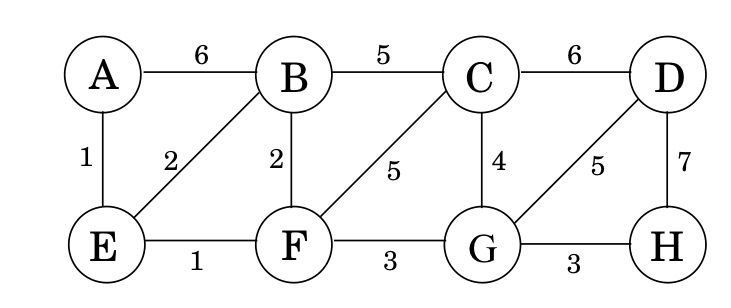
\includegraphics[scale=0.3]{mst_graph_q2.jpg} 
\end{center}
\end{figure}
\begin{solution}
NoMST = \{(D,H), (C,D), (A,B)\} \\ \\ These 3 edges cannot be apart of the MST because of the cut property. There is no cut that you can make that will make (D,H), (C,D), or (A,B) the shortest path going into any of the verticies B,C,D. This is one of the properties that makes Kruskal's algorithm optimal, so if that property is broken, then there's no way any MST can contain any of these edges.
\end{solution}


\end{enumerate}

\end{document}
